\documentclass{article}

\usepackage[left=1in, right=1in, top=1in, bottom=1in]{geometry}

\usepackage{setspace}
\usepackage{fancyhdr}
\usepackage{hyperref}
\usepackage{amsthm}
\usepackage{amssymb}
\usepackage{multirow}
\usepackage{enumitem}
\usepackage{graphicx}
\usepackage{makecell}
\usepackage{booktabs}
\usepackage{titlesec}
\usepackage{amsmath}
\usepackage{pdfpages}
\usepackage{enumitem}
\usepackage{caption}

\setcounter{secnumdepth}{4}

\hypersetup{
    colorlinks=true,     
    urlcolor=magenta
}

\renewcommand{\qedsymbol}{\rule{0.7em}{0.7em}}

\newlength\tindent
\setlength{\tindent}{\parindent}
\setlength{\parindent}{0pt}
\renewcommand{\indent}{\hspace*{\tindent}}
\setlength{\parskip}{0em}

\newenvironment{blockquote}{%
  \par%
  \vskip1em
  \leftskip=2em\rightskip=2em%
  \noindent\ignorespaces}{%
  \par\vskip1em}

\newenvironment{blockquote2}{%
	\par%
	\vskip1em
	\leftskip=4em\rightskip=4em%
	\noindent\ignorespaces}{%
	\par\vskip1em}

\pagestyle{fancy}
\fancyhf{}
\fancyhead[LO]{STA5176}
\fancyhead[RO]{Kyle Ligon}
\fancyfoot[LO]{Chapter 14 and 15}
\fancyfoot[RO]{\thepage}
 
\renewcommand{\headrulewidth}{0.5pt}
\renewcommand{\footrulewidth}{0.5pt}

\begin{document}
\section*{Chapter 14 and 15 Homework}
\subsection*{Due 4-8-2018}
\subsubsection*{Problem 14.8}
\subsubsection*{ (a) Assess ANOVA assumptions using the graph from PROC MIXED.}
The most concerning plot is the scatterplot with an apparent pattern as you increase the Group Mean.  Though, with a wonky residual histogram and Q-Q Plot that is overpredicting at the extremes this data does not appear to fit a trustworthy ANOVA scenario.  
\begin{figure}[h]
\centering
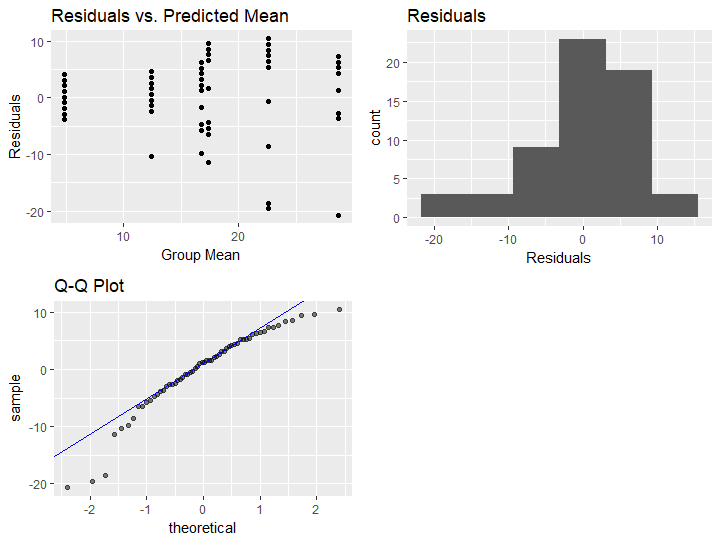
\includegraphics[width = 1.0\textwidth]{ANOVAcheck148.png}
\end{figure}
\subsubsection*{(b) Perform an ANOVA to determine if there is an interaction between the age group and types of products; $\alpha$ = 0:05}
\begin{table}[ht]
\caption{ANOVA Table for Attention Spans}
\centering
\begin{tabular}{l c c c c c}
\hline\hline
Row Names & SS & df & MS & F & P-Value \\ [0.5ex] 
\hline
Main Effect \\ 
\hspace{3mm}Age Group & 1349.6333 & 2 & 674.81665 & 12.868 & 2.67x$10^{-5}$ \\
\hspace{3mm}Products & 1995.2667 & 1 & 1995.2667 & 38.048 & 9.15x$10^{-8}$\\
Interaction \\
\hspace{3mm}(Age Group:Products) & 14.2333 & 2 & 7.1167 & 0.136 & 0.873 \\
Error & 2831.8000 & 54 & 52.4407 \\
Total & 6190.9 & 59 &  \\ [1ex]
\hline
\end{tabular}
\label{table:nonlin}
\end{table}

Check the Interaction, Reject if $F_{Interaction} > F_{\alpha, df_{Interaction}, df_{Error}}$:
\begin{blockquote}
$F_{Interaction} = 0.873 < 3.1682 = F_{0.05, 2, 54}$ \\
Thus, the interaction is not significant and can be removed from the model.  
\end{blockquote}

\subsubsection*{(c) If there is an interaction, create a probability plot for age group and product type and provide an interpretation for the interaction}


Dealing with the Interaction Term
\begin{blockquote}
Since the Interaction term of AgeGroup:Products is not significant ($> F_{0.05, 2, 54} = 3.1682$), we will remove it from our ANOVA model and just look at the Main Effects.
\end{blockquote}


\subsubsection*{(d) If there is not an interaction, remove the interaction term, recompute the ANOVA table, and determine if there are main effects of age group and product type; $\alpha$ = 0:05}

\begin{table}[ht]
\caption{ANOVA Table for Attention Spans without Interaction Term}
\centering
\begin{tabular}{l c c c c c}
\hline\hline
Row Names & SS & df & MS & F & P-Value \\ [0.5ex] 
\hline
Main Effect \\ 
\hspace{3mm}Age Group & 1350 & 2 & 674.8 & 13.28 & 1.91x$10^{-5}$ \\
\hspace{3mm}Products & 1995 & 1 & 1995.3 & 39.26 & 5.60x$10^{-8}$\\
Error & 2846 & 56 & 50.8 \\
Total & 6191 & 59 &  \\ [1ex]
\hline
\end{tabular}
\label{table:nonlin}
\end{table}

Checking to see if the F Statistics Are Greater Than $F_{\alpha, df_{Main Effect}, df_{Error}}$
\begin{eqnarray}
F_{Age Group} = 13.28 > 3.1619 = F_{\alpha, df_{Main Effect}, df_{Error}}  \nonumber \\
F_{Products} = 13.28 > 4.0130 = F_{\alpha, df_{Main Effect}, df_{Error}}  \nonumber 
\end{eqnarray}

\begin{blockquote}
Both the Main Effects are statistically significant therefore, we should move onto Post Hoc testing to look at statistically different pairs.  
\end{blockquote}



\subsubsection*{(e) Report significantly different pairs using Tukey's W and $\alpha$ = 0:05; REMEMBER: if there is an interaction present, we must account for that when performing post-hoc testing}

\subsection*{14.10}

\subsubsection*{(a) Assess ANOVA assumptions using the graph from PROC MIXED.}

\subsubsection*{(b) Determine if there is a difference between gasoline blends using ANOVA for Latin Square; $\alpha$ = 0:05}

\subsubsection*{(c) If there is a difference per part (b), use Tukey's W to determine the significantly different pairs; $\alpha$ = 0:05}

\subsubsection*{(d) From part (c), which blend (or blends) gives the highest gas mileage?}

\subsubsection*{(e) Determine if there is a difference between gasoline blends using ANOVA for completely randomized designs (i.e., ignore the blocking factors); $\alpha$ = 0:05}

\subsubsection*{(e) Compare the MSE from part (b) to the MSE from part (e) - what happens when we ignore the blocking factors? }

\subsubsection*{(f) Which would you say is the appropriate analysis?}

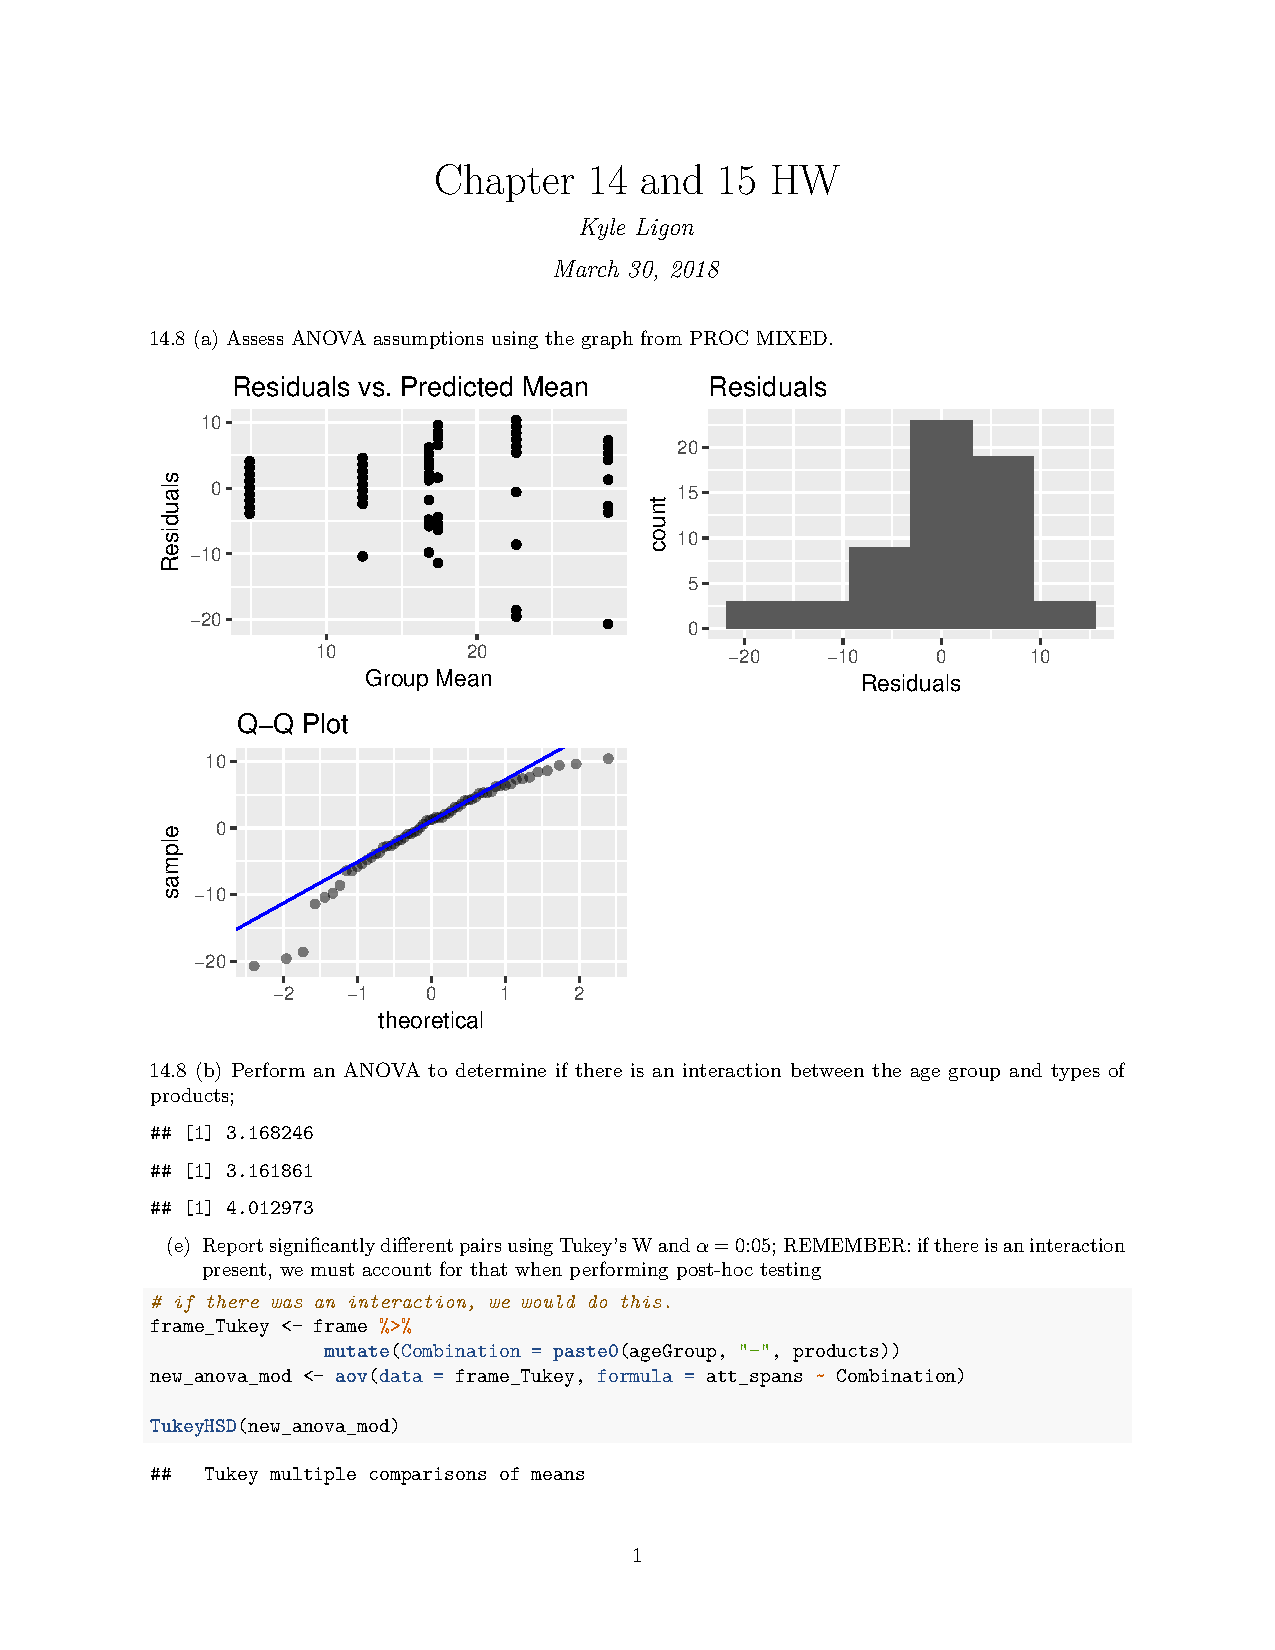
\includepdf[pages=-]{Chapter14_and_15_HW.pdf}

\end{document}















